\chapter{The KANDY Benchmark}
\label{chap:kandybench}

In this chapter we introduce \textsc{KANDY}, a benchmarking framework that can be used to generate a variety of learning and reasoning tasks inspired by Kandinsky patterns. By creating curricula of binary classification tasks with increasing complexity and with sparse supervisions, \textsc{KANDY} can be used to implement benchmarks for Continual and Semi-supervised Learning, with a specific focus on symbol compositionality. The ground truth is also augmented with classification rules to enable analysis of interpretable solutions.
\textsc{KANDY} is publicly released\footnote{\url{https://github.com/continual-nesy/KANDYBenchmark}} as a generator and a collection of ready-to-use datasets.
Experiments of Chapter~\ref{chap:kandyind} and Chapter~\ref{chap:kandycem} will rely on such datasets.
The content of this chapter is adapted from our MLJ journal paper~\cite{lorello2025kandy} and CoLLAs 2024 conference paper~\cite{lorello2024continual}.

\section{\textsc{KANDY} at a glance}%\label{kandy:sec:benchmark}
With respect to the taxonomy introduced in Chapter~\ref{chap:benchnesy}, \textsc{KANDY} can be described as an \textbf{image}-based benchmark, capable of covering \textbf{multiple families of tasks}. \textsc{KANDY} requires \textbf{First-order} expressivity to be solved successfully, it can be employed in \textbf{multiple reasoning directions} (with a particular focus on inductive reasoning), and it discloses data in a \textbf{incremental} fashion, with ground truth knowledge \textbf{given}, but evolving in a \textbf{defeasible} manner over time. 
The following are the main possible use cases of \textsc{KANDY}:
%
\begin{enumerate}
    \item \textbf{Offline vs. Continual Learning.} Data generated by \textsc{KANDY} can be used to compare classical ``offline'' batch-mode learning, where the whole training data is immediately available to the learning agent, with Continual/Lifelong Learning, where data is made progressively available to the learner, with or without repetitions.
    \item \textbf{Independent Tasks vs. Multi-task.} Tasks within a curriculum can be considered independent one from the other (thus training independent classifiers), or they can be jointly addressed in a multi-task setting (thus training a single classifier).% This comparison can be performed both in batch and in continual learning.
    \item \textbf{Curriculum vs. Random Order.} Tasks (and samples) can be shown to the learning agent in the order defined by the user (curriculum) or in a random order. In the former case, the agent is expected to progressively acquire skills to solve tasks of increasing complexity.
    \item \textbf{Supervised vs. Semi-supervised.} Tasks can be fully supervised, as well as sparsely supervised with a customizable criterion, raising the additional challenge of dealing with a semi-supervised data set.
    \item \textbf{Interpretability vs. Explainability.} Tasks and samples are paired with symbolic ground truth annotations, allowing to compare interpretable-by-design systems and post-hoc explanations.%By providing the ground truth of the rules that are used to define each binary classification problem, KANDY allows to compare systems that learn interpretable rules (which thus can be diagnosed) with approaches that are not interpretable by design, but whose solutions can only be inspected with XAI techniques, a posteriori.
\end{enumerate}
%In the following we describe the main building blocks of the framework, supported by Figure~\ref{kandy:fig:example-kandy}, and two curricula that we release as open challenges. 
%Further details are provided in the supplementary material, while several usage-oriented details are  reported in the KANDY code repository, where we publicly share the data generator, our curricula, and code for running experiments with neural and symbolic baselines: \url{https://github.com/continual-nesy/KANDYBenchmark}.


\begin{figure}
\centering
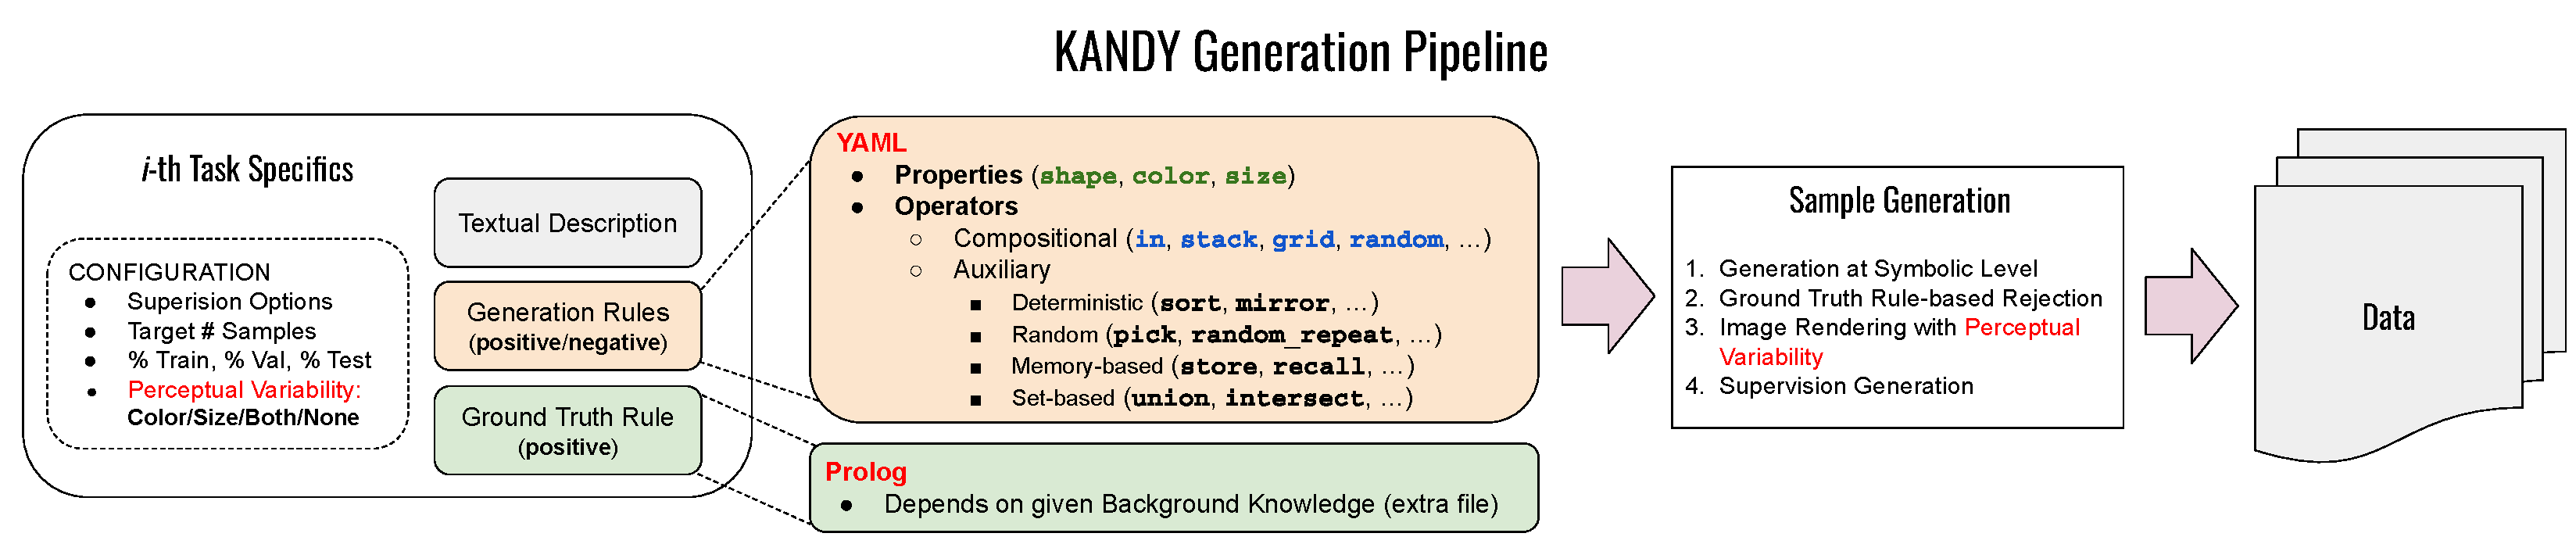
\includegraphics[width=1.0\textwidth]{imgs/kandy/Fig1a.pdf}
\vskip 4mm
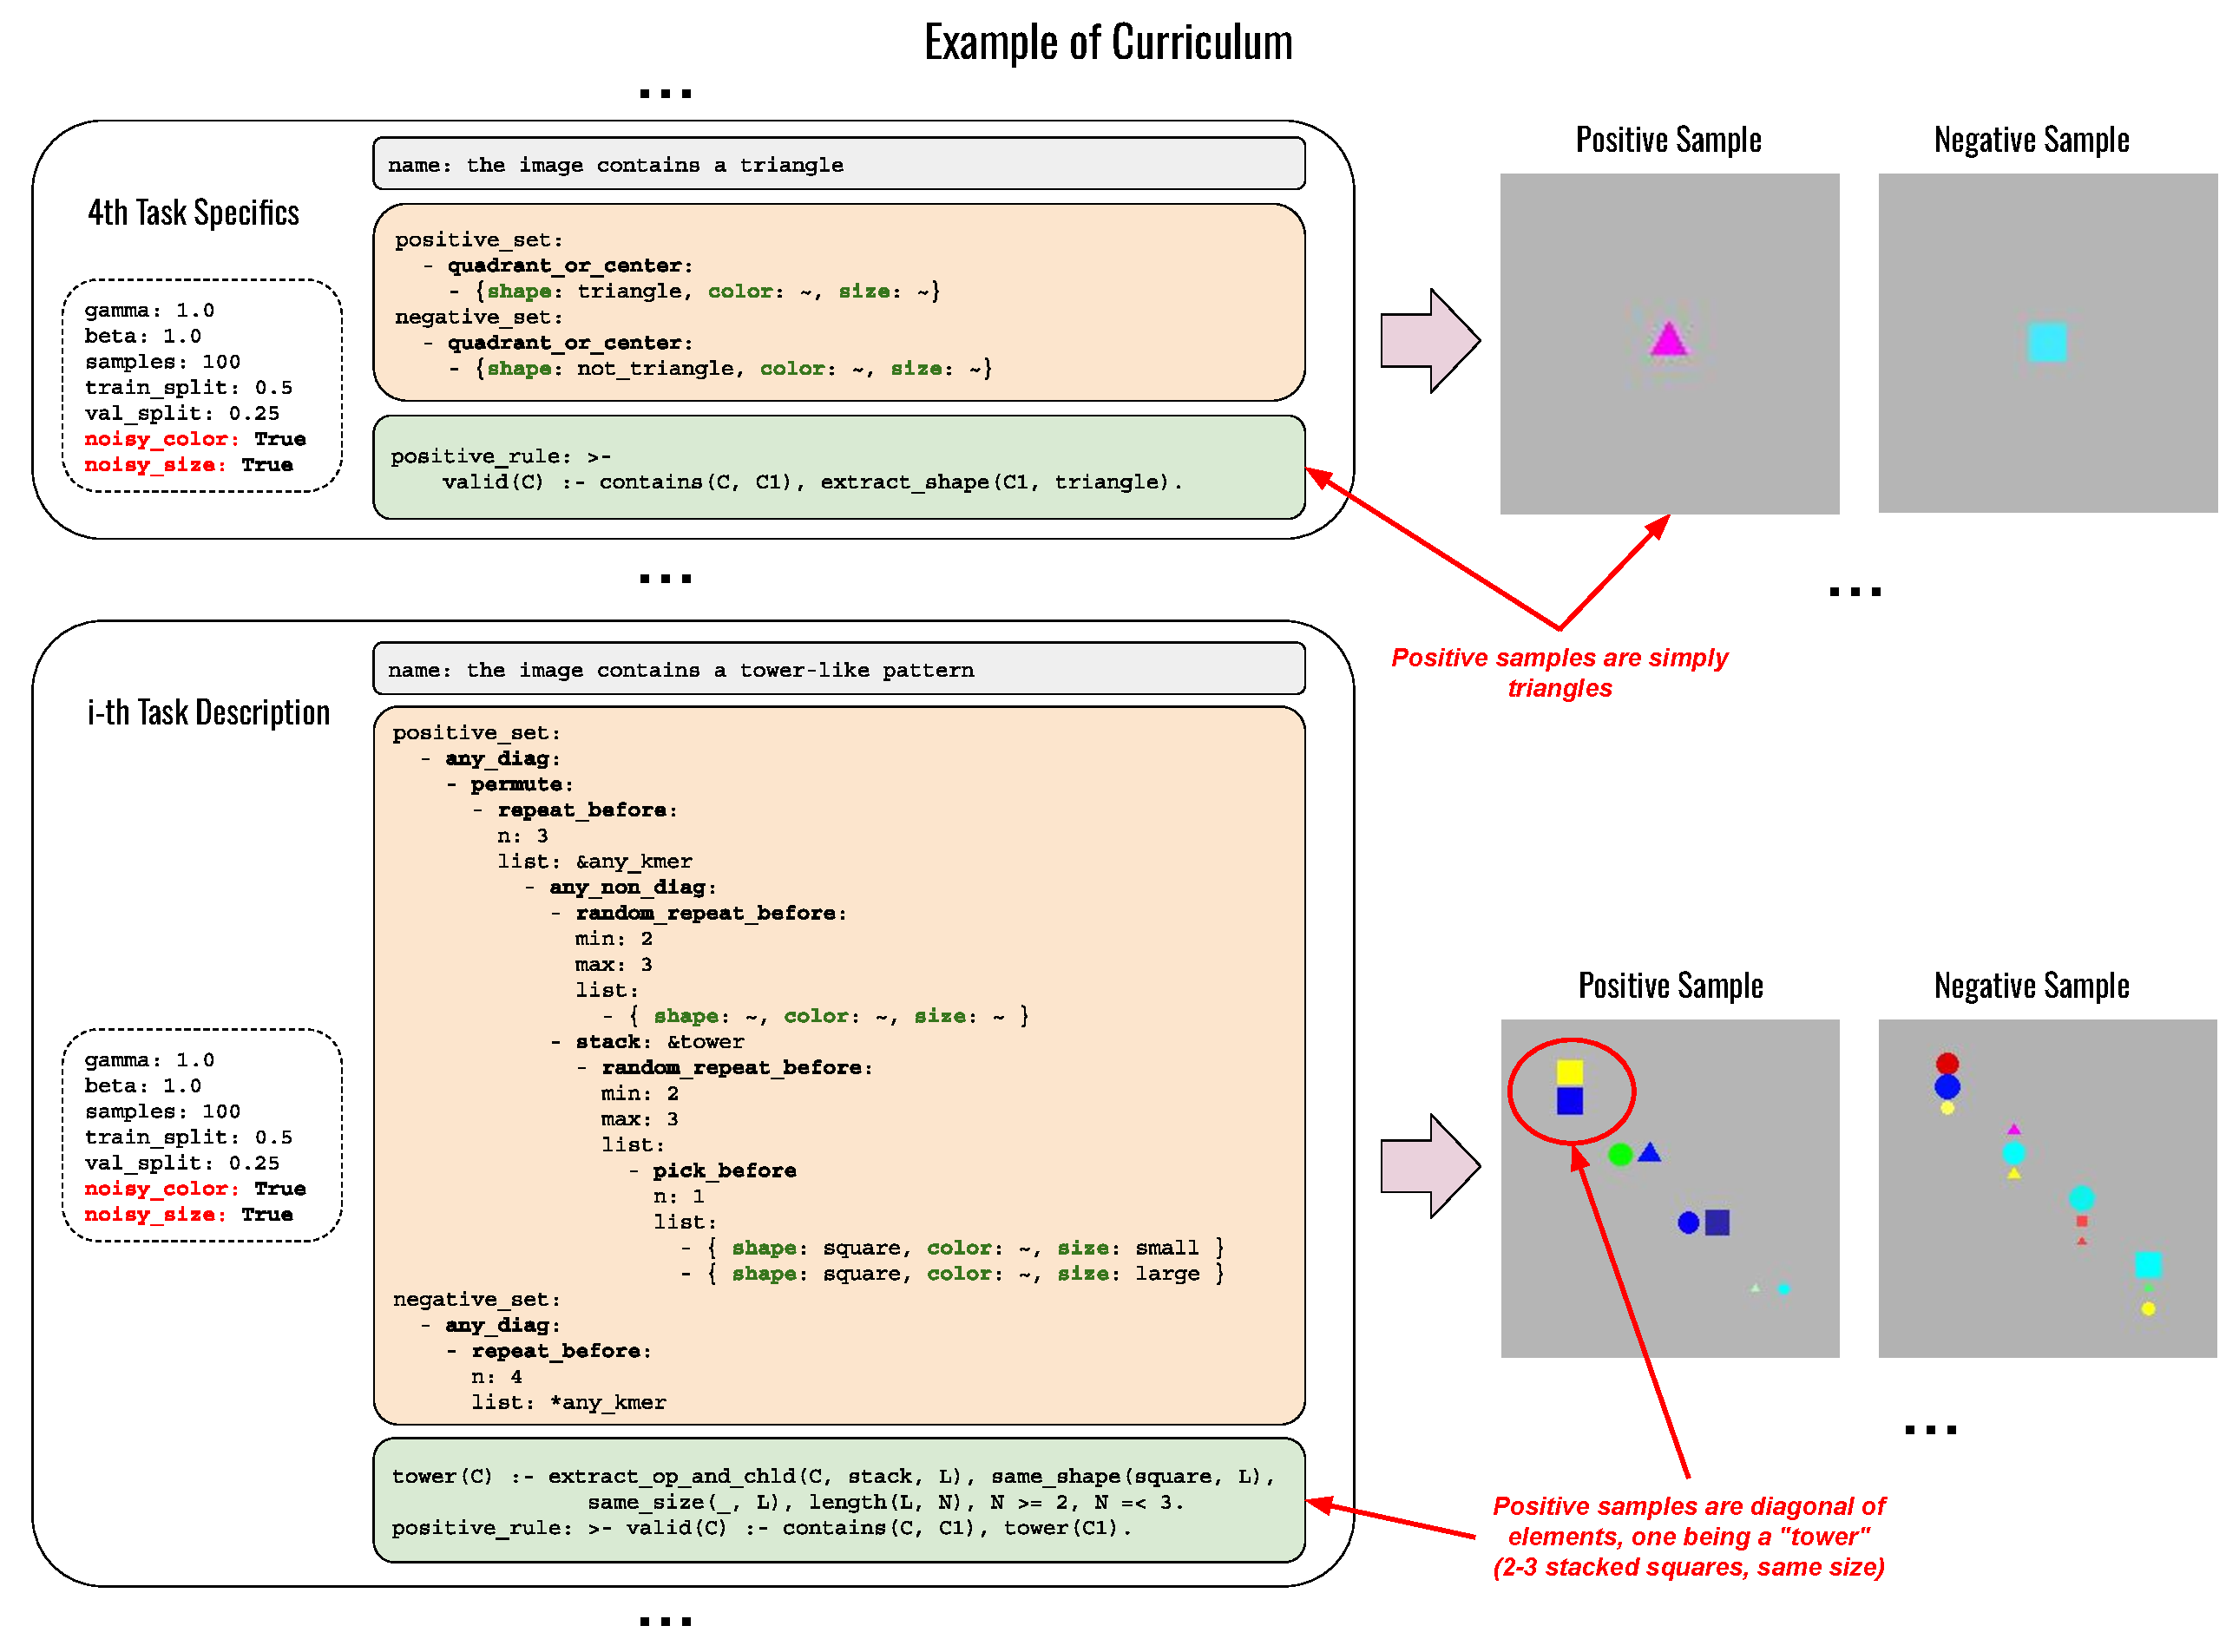
\includegraphics[width=\textwidth]{imgs/kandy/Fig1b.pdf}
\caption[KANDY generation pipeline]{\textit{Top:} Overview of the KANDY generation pipeline: the user provides task specifics and data is generated. Positive and negative sets are defined via symbolic representations and rendered into synthetic images. The ground truth rule is a propositional clause that can be used to reject samples, and thus explains the task. \textit{Bottom:} Example of two tasks from a curriculum generated with KANDY. \label{kandy:fig:example-kandy}}
\end{figure}

\section{Data Generation}\label{kandy:sec:generation}
%\input{src/generator}

Curricula in \textsc{KANDY} are defined in YAML format as lists of tasks. Each task is characterized by two mandatory descriptions of the positive and negative sets as {\it generation rules}, in the form of lists of perceptual trees, where leaves are atomic shapes, and intermediate nodes are annotated with {\it compositional operators}.  In order to avoid the exhaustive enumeration of each image sample, {\it auxiliary operators} (e.g., randomly selecting between multiple options, copying a subtree in a different location, etc.) can be used to expand the list programmatically.
Optionally, each task can also define a {\it ground truth rule}, which is a Prolog-interpretable $\texttt{valid/1}$ predicate (built on some background knowledge). Collectively, generation and ground truth rules describe the task (Figure~\ref{kandy:fig:example-kandy}, top).
KANDY yields synthetic images containing compositions of simple geometric shapes with several configurable properties: \textit{color}, \textit{shape}, and \textit{size}. %, relative position. 
%Tasks consist in binary classification problems defined by positive and negative sets, optionally filtered by a symbolic rule at sampling time. Curricula are defined as sequences of tasks. 
%
Images correspond each to a perceptual tree from the generation rules, and they are iteratively generated by a sampling procedure. If the ground-truth rule is specified, incoherent trees (i.e., samples from the positive set violating the rule and samples from the negative set satisfying it) are discarded.
%Moreover, the generator allows to corrupt task indices, to investigate the effect of task selection errors in multi-task or continual learning settings.



\paragraph{Sample Generation.} 
Task generation rules are symbolic representations that are handled by \textsc{KANDY} in the form of collections of trees (forests). When rules are parsed and a new tree is generated, it is checked against the set of previously generated symbols (to avoid redundancy) and, optionally, against the ground-truth rule, to guarantee consistency between the generation rules and the ground-truth information. 
%
Then, the data generator tries to build samples that are inherently different at the symbolic level. %, thus strongly emphasizing the symbolic nature of the generation process. 
Symbol sets are built by sampling trees from either positive or negative generation rules, and by grounding their leaves.
Since rules might involve non-deterministic attributes,\footnote{Any value (\texttt{\textasciitilde}), negation (\texttt{not\_*}), and disjunction (\texttt{a|b|\dots|k}).} a value is randomly assigned to each of the ungrounded attributes. %selects their values.
Finally, perceptual variability is introduced when the image is generated from its symbolic representation, slightly altering size and color. 
%
%A task is defined by two sets (positive and negative) of symbolic representations, in the form of forests (collections of trees). For each task, when a new tree is generated, it is checked against the set of previously generated symbols (to avoid redundancy) and, optionally, against a user-defined rule (to guarantee consistency). %%Such rule is defined as a Prolog-interpretable $\texttt{valid/1}$ predicate.
%
%A sample is rejected either if it has already been generated (rejection by repetition), or if its sampling set is discordant with the rule (i.e., a sample from the positive set does not satisfy the rule, or a sample from the negative set satisfies it, rejection by rule). The maximum number of rejections is governed by a patience hyper-parameter.
The sampling process is repeated until the target number of examples is produced, unless too many samples are rejected consecutively (controlled via a patience hyper-parameter). In such case, the target size is achieved at rendering time by sampling trees with replacement.
%
%Symbol sets are built by sampling trees from either positive or negative sets, and grounding their leaves.
%Grounding randomly selects values for non-deterministic attributes: any (\texttt{\textasciitilde}), negation (\texttt{not\_*}) , and disjunction (\texttt{a|b|\dots|k}).
%
Symbols are then rendered as images and disjointly split into training, validation and test sets.
%Training, validation and test sets are then built by rendering each symbol into an image, and then disjointly splitting samples according to the target percentages. 
%Examples of generation rules, ground truth, and generated data for two different tasks of a curriculum are given in Figure~\ref{kandy:fig:example-kandy} (bottom).
Figure~\ref{kandy:fig:example-kandy} (bottom) exemplifies generation rules, ground truth, and generated data for two different tasks of a curriculum. In the first task, positive examples are simply images containing triangles of any size and color. In the second task, the property shared by positive examples is more complex, since it consists in a diagonal of objects, one of which must be a tower, i.e., a stack of 2-3 squares of the same size. As negatives also contain diagonals, displacement alone is insufficient to characterize the positive set.


%In the final phase, exactly $\text{target samples} \cdot \text{split percentage}$ are generated: if patience was not exhausted in the first phase, sampling is performed without replacement (and symbols are guaranteed to be unique in every split), otherwise, sampling is performed with replacement.
%In the former case, splits are naturally balanced between positive and negative labels (thanks to the 0.5 probability of choosing between positive and negative sets), while in the latter, label distribution will be unbalanced in favor of the label with the highest symbolic variability: if both distributions are exhausted after reaching the target number of samples, imbalance will reflect the ratio of variability between positive and negative sets, if either is still capable of providing new samples, label distribution will be a poor proxy of symbol distribution.

\paragraph{Image Rendering.}
%
%\textcolor{red}{Questi valori sono quelli di KANDY, ma il generatore può essere configurato con valori arbitrari (inclusi il colore di sfondo e il numero di classi di colore e dimensione)}
%\textcolor{red}{@MARCO: da rivedere.}
%Perceptual details: these considerations apply AFTER symbol generation, thus they do not affect purely symbolic systems, such as the ILP baselines. AAAAAAAAAA
%
Images are drawn at a customizable resolution after symbol generation and sample rejection phases. The background color can be customized as well, and shapes can take any color from a discrete set of configurable values.
%
Similarly, the size of atomic shapes can be controlled by defining a set of sizes of interest, and such a size is not a function of the level of the hierarchy to which atomic shapes belong.\footnote{If the drawing area is too small to draw an atomic shape, overlaps can happen in crowded or highly hierarchical scenes.}
%
Both size and color can be injected with configurable noise, to implement the already mentioned initial perceptual augmentation.

%We deemed alternative approaches not viable, namely, recursively reducing atomic shapes would have caused the risk of unrecognizable shapes with deep hierarchies and the inhability of assigning clear labels to different sizes (as a small triangle on the first level of a hierarchy could be mistaken for a large triangle on the second level, and so on), and cropping would have, likewise, caused unrecognizable shapes (with the degenerate case of bounding boxes smaller than the largest inscribed square in a triangle/circle degenerating to a square).

%\subsection{Task creation: design choices and constraints}
%
%Explain the criteria that drive the process of creating tasks, and especially tasks with incremental complexity. Here explain the constraints and the rationale that we have used to construct the 2/3 data sets that we release.

\paragraph{Supervisions.} \textsc{KANDY} allows to sparsely attach supervisions in the generated curricula of tasks, a process which is modeled by a customizable law $f$. For each task, samples are sorted accordingly to the way the were generated, and the supervision law is function of the sample index $t$, scaled in $[0, 1]$ (i.e, $t=0$ is the first sample of the task and $t=1$ is the last one). %which is instantiated for each (non-rejected) sample in a given task of the curriculum (different tasks have their own private In progression variable). 
\textsc{KANDY} implements an exponential decay law which is evaluated for each sample, $f(t) = \gamma \cdot e^{-\sigma \cdot t}$, where $\sigma = \log(\gamma \cdot \beta^{-1})$ and $\gamma, \beta \in [0, 1]$ are hyper-parameters which can be independently defined for each task in the curriculum.
Function $f(t)$ is monotonically decreasing and has boundary values $f(0) = \gamma$ and $f(1) = \beta$.
Then, a binary random variable is sampled with probability $P_t = f(t)$. \textsc{KANDY} attaches supervised annotations to the image if and only if such binary random variable returns a positive outcome.
%With this strategy, supervisions are more frequent at the beginning of the learning process, while being gradually reduced through time.
This simple strategy effectively schedules sporadic supervisions in a way which is most beneficial for the learning process: supervisions are more abundant at the beginning, when parameters are far from optimal, and are gradually reduced as learning progresses.
We claim that this strategy offers two main advantages: with only two hyper-parameters it allows to govern the exploration-exploitation trade-off (by assigning different importance to the unsupervised and supervised objectives, respectively, at different time steps), and, in learning settings where annotations are not easily available, it allows to allocate limited labels in an effective order.

\paragraph{Compositional Operators.} Compositional primitives are used to model the generation rules (Figure~\ref{kandy:fig:example-kandy}, top) that allow \textsc{KANDY} to recursively place and display children objects (either atomic shapes or other compositional primitives) within the image, as a function of the bounding boxes of such objects. %, by computing bounding boxes of the appropriate dimensions and positions.
%
%receive from their caller (which is either the root sampler or a compositional primitive above) a bounding box, inside which they can draw: it is their responsibility to compute a new, smaller, bounding box for each of their children for the recursive step, and then draw their returned image at the correct location.
%Each compositional primitive reduces bounding boxes in a way linked to its semantics, however, in every case, bounding boxes have a lower bound equal to the space required to draw the largest atomic object, this limit can cause overlaps when composing too many objects, or drawing deep hierarchies.
%
The simplest operator is called \texttt{in} and it draws a child object at the center of the drawing area.
%
Similarly, operators \texttt{quadrant\_ul, quadrant\_ur, quadrant\_ll, quadrant\_lr}
%do not alter the children bounding boxes, but shift their center to one of the four corners of the parent bounding box, resulting in overlapped, but de-centered, objects.
position the bounding box of an object in one of the four quadrants of the drawing area.
%
The \texttt{random} operator draws children objects at random positions, using greedy sample rejection to avoid overlapping with previously drawn shapes.
%exploits a greedy rejection sampling (using the same patience hyperparameter of the general algorithm) to try producing non-overlapping objects. Each child is drawn at a random position, with the whole space available, but if the pixel-wise intersection of the current child and the previously drawn ones is not empty, the current child's position is rejected and resampled. For simplicity there is no backtracking on already drawn children, this implies that the probability of collisions gets increasingly higher as drawing progresses.
%
Operators \texttt{stack} and \texttt{side\_by\_side} equally split the drawing area available for each child along their primary axis (vertical for \texttt{stack} and horizontal for \texttt{side\_by\_side}), while preserving the secondary axis.
%The secondary axis is not split, e.g., a parent bounding box of $384 \times 384$ pixels is split among 10 \texttt{stack}ed children as 10 $384 \times 38$ bounding boxes.
Objects are drawn left-to-right for \texttt{side\_by\_side} and top-to-bottom for \texttt{stack}.
The variants \texttt{stack\_reduce\_bb} and \texttt{side\_by\_side\_reduce\_bb}, instead, also reduce the secondary axis size. %These four operators can be combined to produce perceptually (and possibly semantically) different types of compositions, such as crosses (e.g., \texttt{stack(A, side\_by\_side(B, C, D), E)}), or ``temporal sequences'' (e.g., \texttt{side\_by\_side\_reduce\_bb(stack(A, B, C), stack(B, C, A), stack(C, A, B))}).
%
The \texttt{diag\_ul\_lr} operator positions children objects from the upper-left corner towards the lower-right, while \texttt{diag\_ll\_ur} arranges childred objects from lower-left to upper-right. %Bounding boxes for diagonal operators are computed by dividing both axes by the number of children. %, e.g., a parent bounding box of $256\times 128$ pixels is split among 5 children as $51\times 26$ pixels bounding boxes.
%
The \texttt{grid} operator computes the smallest $n$ such that $n^2 \leq \#\mathrm{children}$ % and divides the bounding box accordingly. 
and children objects are drawn on an $n \times n$ grid from left to right, filling one row at the time, from top to bottom. Grids are incomplete in case the number of children is not a perfect square.

\paragraph{Auxiliary Operators.}
%
%\textcolor{blue}{L. Abbiamo perso la parte importante degli operatori composizionali, questi descritti sono syntactic sugar per semplificare la definizione dei task...}\textcolor{red}{Non ci ero ancora arrivato, ho aggiunto sotto la 3.1.4 come placeholder...}
%
%Besides the set of primitives defined in the previous section, our framework allows to specify, when designing tasks, also additional operators that are easier to use for humans to build symbolic representations.
\textsc{KANDY} also includes additional human-understandable auxiliary operators that simplify the definition of tasks.
%
These operators are list expansion primitives, which allow for compact definitions, mapping lists into other lists containing only atomic shapes and compositional operators.\footnote{For greater flexibility, list expansions are performed twice, operators whose name includes the \texttt{before} suffix are expanded before grounding the sample tree, while every other operator is expanded after grounding.}
%
%We propose two flavors of list expansion operators: one is applied before grounding atomic shapes, the other after grounding. For instance, given the same input list $[\text{any shape}]$ to the repeating operator applied before or after grounding yields different results: $\text{repeat}(2, [\text{any triangle}]) = [\text{small yellow triangle}, \text{small yellow triangle}]$, compared to $\text{repeat\_before}(2, [\text{any triangle}]) = [\text{small yellow triangle}, \text{large blue triangle}]$.
%We provide a complete description of each operator in the code repository. 
In particular, KANDY provides four families of list expansions: (i.) \textit{deterministic}, (ii.) \textit{random}, (iii.) \textit{memory-based}, and (iv.) \textit{set-based}. %, see also Figure~\ref{kandy:fig:example-kandy} (top).
%
\textit{Deterministic} operators (e.g., sorting or mirroring a list) always produce the same output, for a given input. %, note however that as grounding is always a random process, the final outcome will be randomized if deterministic before-grounding operators are used.
%
\textit{Random} operators may produce different results on the same inputs; their behavior can be parameter-free (e.g., random permutation), or controlled by parameters (e.g., random repetition within a range of values).
%
There are three \textit{memory-based} operators: \texttt{store} and \texttt{store\_before} return the input list itself, but they have the side effect of memorizing it and associating it to a text alias; \texttt{recall} (which can only be applied after grounding, unless in combination with set operators) takes an alias and returns the list previously associated to it.
%
\textit{Set-based} operators have special requirements, as they can only take lists of non-grounded atomic shapes or recalled atomic shapes stored before grounding. They produce a single atomic shape output which is the left-associative application of the set operator to the entire list.\footnote{e.g., $\texttt{intersect}([\texttt{any triangle}, \texttt{any non red}, \texttt{any large object}]) \mapsto \texttt{any triangle} \cap \texttt{any non red} \cap \texttt{any large} = \texttt{large non red triangle}$.} We note that proper care should be taken with intersections, as empty output sets are invalid.

\paragraph{Generation Example.} Let us consider the bottom example of Figure~\ref{kandy:fig:example-kandy}.
Both positive and negative sets possess a single element in their list; however, as they contain \textit{auxiliary operators}, these lists will be expanded during sampling.\footnote{Expansion is performed virtually while sampling, to avoid a combinatorial explosion in memory.}
%
First, as the specification is loaded, the YAML engine will process the anchors (\texttt{\&any\_kmer} and  \texttt{\&tower}), associating their labels to a specific subtree, which is copied syntactically every time the corresponding aliases (\texttt{*any\_kmer}, in the negative set, and \texttt{*tower}, in different tasks not shown in the image) are referenced. This step is performed transparently by the YAML engine before \textsc{KANDY} begins parsing the specification.
%
Then, the sampler performs a first bottom-up pass on each tree, and replaces each \texttt{\_before} auxiliary operator (for the positive set these are: \texttt{pick\_before}, \texttt{random\_repeat\_before}, \texttt{random\_repeat\_before}, \texttt{repeat\_before}). For example, the \texttt{pick\_before} subtree is replaced by selecting a single (\texttt{n: 1}) entry from the list of  provided options.
At this point the positive set will have two trees, one where a leaf is replaced by \texttt{\{shape: square, color: \textasciitilde, size: large\}}, and the other with \texttt{\{shape: square, color: \textasciitilde, size: small\}}. Let us  assume the sampler has selected the first one.
%
In the next step, \textit{non-deterministic attributes} are grounded with one of the possible values. For instance, the leaf \texttt{\{shape: square, color: \textasciitilde, size: large\}} can be grounded with any of the six available colors defined in the global configuration section of the YAML file, for  example, \texttt{\{shape: square, color: yellow, size: large\}}.
%
Finally, the sampler performs a second bottom-up pass, resolving each remaining auxiliary operator (for the positive set, \texttt{any\_non\_diag}, \texttt{permute}, \texttt{any\_diag}, in this order). At this point the original sets (containing a single tree each) virtually contain every possible grounding of perceptual trees and the sampler has selected one from either the positive or negative set. Let us assume the following has been sampled from the positive set:
\vskip 2mm
\begin{verbatim}
diag_ul_lr:
  stack:
    - {shape: square, color: yellow, size: large}
    - {shape: square, color: blue, size: large}
  side_by_side:
    - {shape: circle, color: green, size: large}
    - {shape: triangle, color: blue, size: large}
  side_by_side:
    - {shape: circle, color: blue, size: large}
    - {shape: square, color: blue, size: large}
  side_by_side:
    - {shape: triangle, color: green, size: small}
    - {shape: circle, color: cyan, size: small}  
\end{verbatim}
\vskip 2mm
The ground-truth rule (green box Figure \ref{kandy:fig:example-kandy}, bottom) checks whether the sample should be accepted, by looking for a subtree ($\texttt{contains/2}$) satisfying the predicate $\texttt{tower/1}$. As the tree is indeed valid (the first \texttt{stack} contains two squares of the same size), the image can finally be generated, by introducing small perceptual variability in color and size. The result is the  positive image in the bottom part of Figure \ref{kandy:fig:example-kandy}.


%\subsection{Possible usages and modalities}

%Explain the scenarios in which the benchmark can be used: batch vs. continual, single task vs. multi-task, curriculum vs. random. Also mention the interpretability of results (explanations) as an additional task.


\section{Released Datasets}\label{kandy:sec:curricula}
%\subsection{Released curricula}\label{kandy:sec:curricula}
%As illustrated in the previous subsections, KANDY is a benchmarking framework, that can be exploited to generate novel benchmarks with specific characteristics chosen by developers. Nevertheless,
%To show the potential of KANDY and to issue a challenge that could be taken up by several AI communities, % (e.g., NeSy AI and continual learning), 
%we release two benchmarks in the form of curricula of tasks, that showcase the features available to the end-user. We name the two curricula {\it Easy} and {\it Hard}, due to the different complexity of the involved tasks.
In this section we describe the \textsc{KANDY} datasets released publicly. These consist of (i.) two \textit{temporal induction} datasets, (ii.) two collections of \textit{Bongard problems}, and (iii.) two \textit{concept discovery} datasets.
%
Each sample is a $224 \times 224$ RGB image annotated with: task ID, binary label, supervision state (whether the label should be used in training or if the sample should be treated as unsupervised), and symbolic representation. % (whether it should be considered a supervised sample or whether its label should be used only for evaluation) and the symbolic structure used to generate it.
The symbolic representation is a recursive dictionary of lists representing a tree, i.e., the perceptual tree, as created in the sample generation stage. %, where keys are nodes annotated with compositional operators and values are children. Leaves are dictionaries in the form \texttt{\{shape: SH, color: CO, size: SZ\}}, and they represent atomic objects. 
Concept discovery datasets are additionally annotated with ground truth Boolean concepts generated by Prolog rules applied to each sample.
No list expansion operators appear in symbolic annotations.
%
Atomic objects can be {\it small} or {\it large} ($10 \times 10$ and $25 \times 25$ pixels, respectively), and they can take any of six colors ({\it red}, {\it green}, {\it blue}, {\it cyan}, {\it magenta} and {\it yellow}). Object sizes are corrupted by additive uniform noise in the range $\pm[0, 2]$ pixels, and color is corrupted by zero-mean Gaussian noise in HSV coordinates ($\sigma_H = 0.01, \sigma_S = 0.2, \sigma_V = 0.2$). These values were hand-picked to preserve perceptual boundaries (e.g., humans still perceive the maximally corrupted ``red'' as such). Background is set to gray.


\paragraph{\textsc{KANDY-Induction-1}.} This curriculum consists of $20$ elementary tasks with limited annotations ($100$ samples for each task, split into $50$ training, $25$ validation, and $25$ test samples).
Tasks $0$ to $8$ contain a single object and introduce basic (atomic) shapes ($0$-$2$) and color ($3$-$8$). % (circles, triangles and squares) and color (red, green, blue, cyan, magenta, yellow). 
Positive instances contain an object possessing some target attributes, while negative ones contain an arbitrary object.
%
Tasks $9$ to $12$ introduce simple spatial relations between multiple objects. Namely, in such tasks the rightmost object in a positive sample is always a {\it red triangle}, presented in an increasingly complex context: along with an arbitrary object (task $9$), with multiple arbitrary objects ($10$), multiple objects, one of which is a {\it circle} ($11$), and multiple objects, one of which is {\it blue} ($12$). %\textcolor{red}{We expect a neural network to learn the base feature at task 9 and reuse it for subsequent tasks, given the limited amount of training samples? ML: NON FAREI QUI CONSIDERAZIONI SUI MODELLI.}
%
Tasks $13$ and $14$ present complex inter-object relations without confounders: positives in task $13$ consist of a {\it triangle} and a {\it square} of the same color, positives in task $14$ are {\it palindromes of three objects} (i.e., A B A displaced horizontally).
%
Task $15$ to $19$ introduce ``higher order'' objects, which will be reused for the \textsc{KANDY-Induction-2} curriculum. These objects are (extremely abstract) representations of: {\it houses} (a square below a triangle), {\it cars} (two side-by-side circles of the same size), {\it towers} (two or three stacked squares of the same size), {\it wagons} (two or three side-by-side squares of the same size), and {\it traffic lights} (red, yellow and green circles of the same size stacked). Negative samples are perceptually similar to positives, but violate the ground truth rules. %in this last group of tasks are composed of objects with the same structure as the positives, but violating the given rule (e.g., negatives for the towers task are a stack of two or three arbitrary objects, possibly including squares of different sizes).


\paragraph{\textsc{KANDY-Induction-2}.} This curriculum consists of $18$ tasks requiring complex, incremental reasoning capabilities, designed to be challenging for both neural and symbolic methods.
We provide four versions of this curriculum: small fully supervised ($100$ samples per task, $80$ training, $10$ validation, $10$ test samples), large fully supervised ($1000$ total, $800$ train, $100$ validation, $100$ test samples), and two large versions with sparse annotations (both with $1000$ samples, one has fixed $\gamma=\beta=0.5$ probability of supervision, the other has a decay schedule from $\gamma=0.8$ to $\beta=0.2$ probability).
%, while preserving an incremental nature.
%
Tasks $0$ to $3$ introduce uniform k-mers of two and three objects with a common property. % (these tasks are an extension of task 13 from Easy).
%
Positives in tasks $4$ to $8$ contain the objects introduced at the end of the \textsc{KANDY-Induction-1} curriculum, along with confounders (which were not present in \textsc{KANDY-Induction-1}).
%
Tasks $9$ to $11$ introduce hierarchical reasoning, with a universally quantified rule applied to each of the groups within a grid. Positives of task $9$ contain a {\it grid} whose elements are displaced in {\it diagonal}, such that it exists a {\it shared shape} in every group (e.g., each contains a square). Likewise, in task $10$ the rule universally quantifies the existence of a color and, in task $11$, the rule involves the complex objects defined in the Easy curriculum (thus introducing a 3-level perceptual hierarchy).
%
Task $12$ to $14$ extend the {\it palindrome} task of \textsc{KANDY-Induction-1}: in task $12$, positives are a palindrome of arbitrary size between $3$ and $7$ simple objects, displaced along an arbitrary line (horizontal, vertical or diagonal). Task $13$ introduces the concept of ``{\it pseudo-palindrome}'', defined recursively as a sequence $A B A'$ where $B$ is a pseudo-palindrome, and $A$ and $A'$ share either the same shape or the same color. Positives in task $14$ are pseudo-palindromes where couples $A$ and $A'$ can be either simple or complex objects.
%(for which the previous definition applies), or named objects (which must be identical, following the traditional palindrome definition).
%
Positives in task $15$ contain objects of the same color if their number is {\it odd}, or objects of the same shape if their number is {\it even}.
%
Tasks $16$ and $17$ assess logic implication capabilities on top of complex object recognition. %, with positives in the form ``A implies B''. (i.e., both ``A and B'' and ``not A'' are positive samples).
Positives in task $16$ contain {\it four objects} satisfying $(\text{traffic light} \Rightarrow \text{car}) \vee (\text{house} \Rightarrow \text{tower})$. Task $17$ universally quantifies task 16 on a grid. % of 2-to-4 groups.% extends task 16 on a grid of 2 to 4 groups such as positives have each group satisfying the rule.

%\textcolor{red}{Vincoli reasoning hard? es. dimensione background knowledge + numero predicati regola + numero predicati helper}
%
%\textcolor{red}{Vincoli percettivi hard? es. ammettiamo sovrapposizioni ma solo in named objects riconoscibili?}

\paragraph{\textsc{KANDY-Bongard-1/2}.} Both \textsc{KANDY-Induction} curricula are also released in the form of Bongard problems, with a single image divided in twelve panels for each task. Panels are extracted from the small version of either curriculum, by taking, for each task, the first six positive (rendered on the left portion of the image) and six negative (rendered on the right) samples of the test set, in the order they were generated. Panels are left blank (white) if fewer than six samples of the corresponding label were present in the test set.
We release Bongard problems in three flavors. The first one corresponds to a simple $2\times6$ \textsc{grid} of \textsc{KANDY} images at their original size of  $224 \times 224$ pixels (Figure \ref{kandy:fig:bongard}, left). The other two flavors employ a Foundalis-style\footnote{\url{https://www.foundalis.com/res/diss_research.html}} template (Figure \ref{kandy:fig:bongard}, right), to present \textsc{KANDY} in a way which is perceptually similar to original Bongard problems. \textsc{Foundalis-224} upscales the original template to fit unmodified KANDY images, while \textsc{Foundalis-100} images  are built by downscaling KANDY images to $100\times 100$, which is the panel size in standard Bongard problems.

\begin{figure}
    \centering
    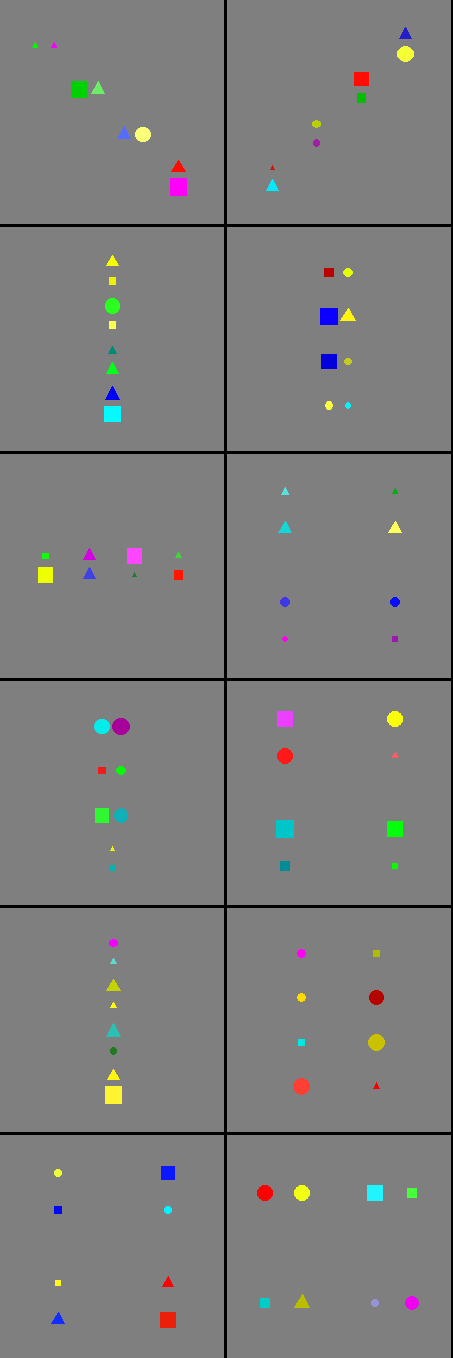
\includegraphics[height=7cm]{imgs/kandy/Fig2a}
    \hfill
    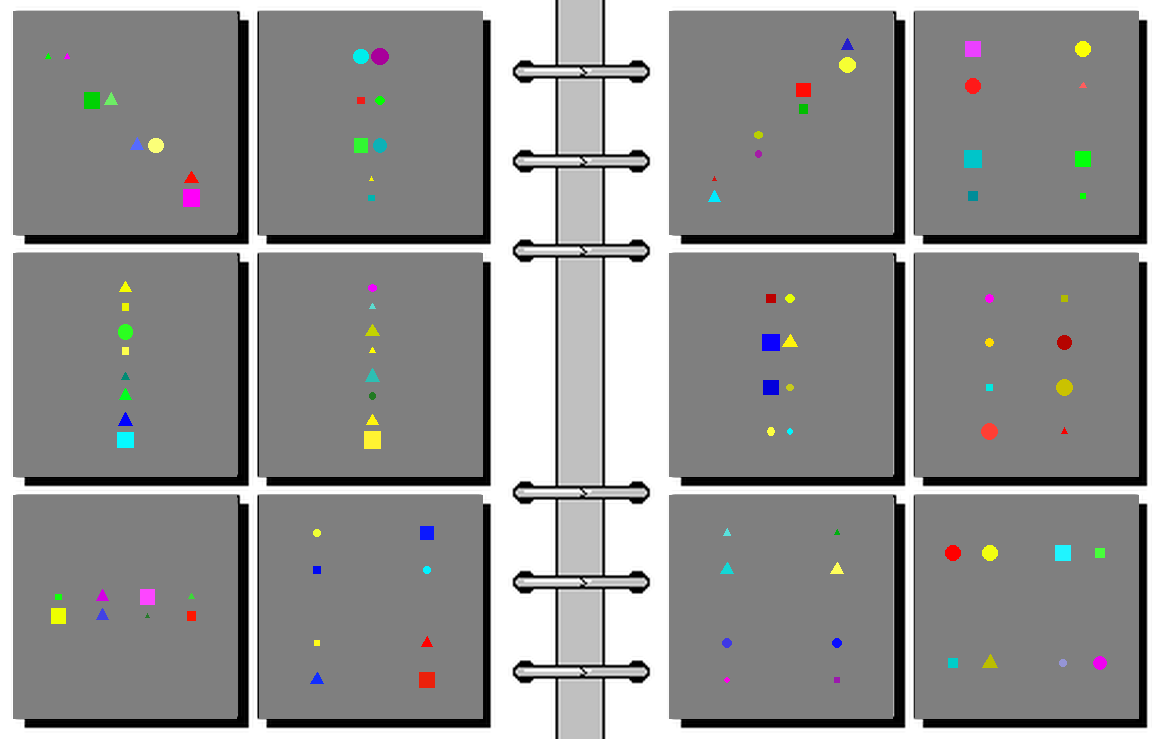
\includegraphics[height=7cm]{imgs/kandy/Fig2b}
    \caption[\textsc{KANDY-Bongard-2} task 4]{\textsc{KANDY-Bongard-2} Task 4, ``There is a house (triangle above a square) somewhere in the image'', in \textsc{grid} (left) and \textsc{Foundalis-224} (right) styles.}
    \label{kandy:fig:bongard}
\end{figure}


\paragraph{\textsc{KANDY-Concepts-1}.}
This curriculum corresponds to \textsc{KANDY-Induction-1}, augmented with concept-level annotations, consisting of elementary attributes (shape, color and size), combined into derived concepts (complex patterns), as highlighted in Table~\ref{cem:tab:kandy_1interactions}. The curriculum is characterized by a warm-up phase (tasks 0 to 8), where only atomic concepts are introduced, followed by a concept-combination phase, in which multiple concepts are combined.

\begin{table}[h]
	\centering
	\resizebox{.7\textwidth}{!}{
		\begin{tabular}{cc|ccc:cccccc:cc}
			\toprule
			\sc Task & \sc Interaction & \multicolumn{3}{c}{\sc Shape} & \multicolumn{6}{c}{\sc Color} & \multicolumn{2}{c}{\sc Size}\\
			&  & \FilledTriangleUp & \FilledSquare & \FilledCircle & \textcolor{red}{\FilledSquare} & \textcolor{green}{\FilledSquare} & \textcolor{blue}{\FilledSquare} & \textcolor{cyan}{\FilledSquare} & \textcolor{magenta}{\FilledSquare} & \textcolor{yellow}{\FilledSquare} & \SmallSquare & \BigSquare \\
			\midrule
			T0   &             & $\exists$    &      &     &      &      &      &      &      &      &     &      \\
			T1   &             &     &  $\exists$    &     &      &      &      &      &      &      &     &      \\
			T2   &             &     &      & $\exists$    &      &      &      &      &      &      &     &      \\
			T3   &             &     &      &     & $\exists$     &      &      &      &      &      &     &      \\
			T4   &             &     &      &     &      & $\exists$     &      &      &      &      &     &      \\
			T5   &             &     &      &     &      &      & $\exists$     &      &      &      &     &      \\
			T6   &             &     &      &     &      &      &      & $\exists$     &      &      &     &      \\
			T7   &             &     &      &     &      &      &      &      & $\exists$     &      &     &      \\
			T8   &             &     &      &     &      &      &      &      &      & $\exists$     &     &      \\
			\hdashline
			T9   &  Binding        & $\exists$    &      &     & $\exists$     &      &      &      &      &      &     &      \\
			T10  &  Binding            & $\exists$    &      &     & $\exists$     &      &      &      &      &      &     &      \\
			T11  &  Binding, AND            & $\exists$    &      & $\exists$    & $\exists$     &      &      &      &      &      &     &      \\
			T12  &  Binding, AND            & $\exists$    &      &     & $\exists$      &           & $\exists$     &      &      &     &    &  \\
			T13  &  Binding           & $\exists$    & $\exists$     &     & \cmark     & \cmark     & \cmark     & \cmark     & \cmark     & \cmark     &     &      \\
			T14  & Complex            & \cmark    & \cmark     & \cmark    & \cmark     & \cmark     & \cmark     & \cmark     & \cmark     & \cmark     & \cmark    & \cmark     \\
			T15  & Pattern & \cmark    & \cmark     &     &      &      &      &      &      &      & \cmark    &  \cmark    \\
			T16  & Pattern &     &      & \cmark    & \cmark     & \cmark     & \cmark     & \cmark     & \cmark     & \cmark     & \cmark    & \cmark     \\
			T17  & Pattern &     & \cmark     &     &      &      &      &      &      &      & \cmark    & \cmark     \\
			T18  & Pattern &     & \cmark     &     &      &      &      &      &      &      & \cmark    & \cmark     \\
			T19  & Pattern &     &      & \cmark    & \cmark     & \cmark     &      &      &      & \cmark     & \cmark    & \cmark     \\
			\bottomrule
	\end{tabular}}
	\caption[\textsc{KANDY-Concepts-1} curriculum]{Concept progression in tasks of \textsc{KANDY-Concepts-1}. When the decision boundary depends on multiple concepts, the type of interaction is summarized by a keyword. Concepts are either existentially quantified ($\exists$) or require task-specific handling (\cmark). The dashed line demarks the point in which we validate our models, as it delimits the boundary between the last task in which elementary concepts are presented and the first complex task.}
	\label{cem:tab:kandy_1interactions}
\end{table}

\paragraph{\textsc{KANDY-Concepts-2}.}
This curriculum, summarized in Table~\ref{cem:tab:kandy_2interactions}, extends \textsc{KANDY-Concepts-1} to a more complex setting. The warm-up phase (tasks 0 to 17) is lengthened to accomodate additional atomic concepts (number of objects and relative alignement of objects within the image), and the concept-combination phase is characterized by concepts which are relations across different objects.
Concepts for task 18 and 19 are simple conjunctions of atomic concepts: a red square, and an blue object combined with another object which is a circle, respectively. Tasks 20 to 24 are characterized by identity relations: every object must have the same shape (20), the same color (21), the same size (22), all the attributes (23), one identical random attribute (24).
The concept associated with task 25 requires every object to have the same color, and at least one of them to be a circle.

\begin{table}[h]
	\centering
	\resizebox{\textwidth}{!}{
		\begin{tabular}{cc|ccc:ccc:ccc:cccccccc}
			\toprule
			\sc Task & \sc Interaction & \multicolumn{3}{c}{\sc Number} & \multicolumn{3}{c}{\sc Alignment} & \multicolumn{3}{c}{\sc Shape} & \multicolumn{6}{c}{\sc Color} & \multicolumn{2}{c}{\sc Size}\\
			&  & \footnotesize one & \footnotesize few & \footnotesize many & \footnotesize diagonal & \footnotesize horizontal & \footnotesize vertical & \FilledTriangleUp & \FilledSquare & \FilledCircle & \textcolor{red}{\FilledSquare} & \textcolor{green}{\FilledSquare} & \textcolor{blue}{\FilledSquare} & \textcolor{cyan}{\FilledSquare} & \textcolor{magenta}{\FilledSquare} & \textcolor{yellow}{\FilledSquare} & \SmallSquare & \BigSquare \\
			\midrule
			T0   &             &  \cmark   &      &     &      &      &      &      &      &      &     &      &      &      &      &      &      &      \\
			T1   &             &     & \cmark     &    &      &      &      &      &      &      &     &      &      &      &      &      &      &      \\
			T2   &             &     & \cmark     &     &      &      &      &      &      &      &     &      &      &      &      &      &      &      \\
			T3   &             &     &      &     & \cmark     &      &      &      &      &      &     &      &      &      &      &      &      &      \\
			T4   &             &     &      &     &      &      & \cmark     &      &      &      &     &      &      &      &      &      &      &      \\
			T5   & OR            &     & \cmark     &      &      &       & \cmark     &      &      &      &     &      &      &      &      &      &      &      \\
			T6   & AND            &     & \cmark     &     & \cmark     &      &      &      &      &      &     &      &      &      &      &      &      &      \\
			T7   &             &     &      &     &      &      &      &  $\exists$    &      &      &     &      &      &      &      &      &      &      \\
			T8   &             &     &      &     &      &      &      &      & $\exists$     &      &     &      &      &      &      &      &      &      \\
			T9   &             &     &      &     &      &      &      &      &      & $\exists$     &     &      &      &      &      &      &      &      \\
			T10  & AND            &     &  \cmark    &     &      &      &      &      & $\forall$     &      &     &      &      &      &      &      &      &      \\
			T11  & OR            &     &      &     &      &      & \cmark     &      &      & $\exists$     &     &      &      &      &      &      &      &      \\
			T12  &             &     &      &     &      &      &      &      &      &      & $\exists$     &      &      &      &      &      &      &      \\
			T13  &             &     &      &     &      &      &      &      &      &      &     & $\exists$     &      &      &      &      &      &      \\
			T14  &             &     &      &     &      &      &      &      &      &      &     &      & $\exists$     &      &      &      &      &      \\
			T15  &             &     &      &     &      &      &      &      &      &      &     &      &      & $\exists$      &      &      &      &      \\
			T16  &             &     &      &     &      &      &      &      &      &      &     &      &      &      & $\exists$     &      &      &      \\
			T17  &             &     &      &     &      &      &      &      &      &      &     &      &      &      &      & $\exists$     &      &      \\
			\hdashline
			T18  & Binding            &     &      &     &      &      &      &      & $\exists$      &      & $\exists$     &      &      &      &      &      &      &      \\
			T19  & AND            &     &      & \cmark     &      &      &      &      &      & $\exists$      &     &      & $\exists$      &      &      &      &      &      \\
			T20  & XOR            &     &      &     &      &      &      & $\forall$     & $\forall$     & $\forall$     &     &      &      &      &      &      &      &      \\
			T21  & XOR            &     &      &     &      &      &      &      &      &      & $\forall$    & $\forall$     & $\forall$     &   $\forall$   & $\forall$     & $\forall$     &      &      \\
			T22  & XOR             &     &      &     &      &      &      &      &      &      &     &      &      &      &      &      & $\forall$     &  $\forall$    \\
			T23  &   Group AND          &     &      &     &      &      &      & $\forall$     & $\forall$     & $\forall$     &  $\forall$   & $\forall$     &  $\forall$    & $\forall$     & $\forall$     & $\forall$     & $\forall$     & $\forall$     \\
			T24  &   Group OR          &     &      &     &      &      &      & $\forall$     & $\forall$     & $\forall$     &  $\forall$   & $\forall$     &  $\forall$    & $\forall$     & $\forall$     & $\forall$     & $\forall$     & $\forall$     \\
			T25  & AND + XOR            &     &      &     &      &      &      &      &      &  $\exists$    & $\forall$    & $\forall$     & $\forall$     & $\forall$     & $\forall$     & $\forall$     &      &      \\
			\bottomrule
		\end{tabular}
	}
	\caption[\textsc{KANDY-Concepts-2} curriculum]{Concept progression in tasks of \textsc{KANDY-Concepts-1}. When the decision boundary depends on multiple concepts, the type of interaction is summarized by a keyword. Concepts are existentially quantified ($\exists$), universally quantified ($\forall$), or require task-specific handling (\cmark). The dashed line demarks the point in which we validate our models, as it delimits the boundary between the last task in which elementary concepts are presented and the first complex task.}
	\label{cem:tab:kandy_2interactions}
\end{table}
